%\paragraph*{}В ходе \hypertarget{ontogenesis}{онтогенеза} происходит рост и развитие организма растения.
\paragraph*{}Рост и развитие -- неотъемлемые свойства любого живого организма.

\paragraph*{}Рост растения, как и любого другого организма тесно связан с таким понятием как \gls{ontogenesis}.
\remember{Термином \gls{ontogenesis} обозначается индивидуальное развитие организма от зиготы или вегетативного зачатка до его естественной смерти.} 

\paragraph*{}В ходе \hypertarget{ontogenesis}{онтогенеза} реализуется наследственная информация организма -- генотип. А под воздействием \hyperlink{question_gen_code}{генов} и конкретных условий окружающей среды формируется фенотип -- совокупность всех признаков и свойств данного индивидуального организма.

\paragraph*{}\note{Необходимо понимать различия между понятиями \Gls{growth} и \Gls{evolution}}

\paragraph*{}\remember{\hypertarget{growth}{\Gls{growth}} -- это необратимое увеличение размеров и массы клетки, органа или всего организма растения, связанное с новообразованием элементов составляющих его структуру.

\hypertarget{evolution}{\Gls{evolution}}, же -- это качественные изменения в структуре и функциональной активности растения и его частей в процессе онтогенеза. Возникновение качественных различий между клетками, тканями и органами получило название \gls{diferintation}}

\note{Рост и развитие тесно взаимосвязаны, однако не всегда развитие сопровождается ростом. Например растение может долгое время расти и при этом находится в одной и той же фазе развития, например ювенильной. В то же время, в процессе онтогенеза растение может уменьшать свои размеры, например, когда осенью у двулетних растений отмирает надземная часть побега. Кроме того, быстрый рост может сопровождаться медленным развитием и \hyperlink{rapid_growth}{наоборот}}

\paragraph*{}Процессы роста и развития происходят на всех уровнях организации:

\begin{enumerate}
	\item Субклеточном;
	\item \hyperlink{cell_ontogenesis}{Клеточном};
	\item \hyperlink{plant_ontogenesis}{Организменном};
\end{enumerate}

\subsection*{Особенности роста клеток}

\paragraph*{}Различают следующие фазы \hypertarget{cell_ontogenesis}{\gls{ontogenesis}а} растительной клетки:

\begin{enumerate}
	\item Эмбриональная фаза;
	\item Фаза растяжения;
	\item Фаза дифференцировки;
	\item Фаза зрелости;
	\item Старение и смерть;
\end{enumerate}


\subsubsection*{Эмбриональная фаза}

\paragraph*{}Находясь на эмбриональной стадии развития клетка растения способна к делению. При этом, период существования клетки от момента её образования путём деления материнской клетки до собственного деления или гибели носит название \gls{cellCycle} (\ris \ref{cell_cykle}) Эмбриональная фаза или митотический цикл клетки делится на два периода: 

\begin{enumerate}
	\item Собственно \hyperlink{question_mitosis}{деление клетки} или  \gls{mitosis}, длительностью 2-3 часа; 
	\item Период между делениями или интерфаза длительностью 15-20 часов. В свою очередь интерфаза подразделяется на несколько периодов: 
	\begin{enumerate}
		\item Пресинтетический -- период G1 (от англ. gap – интервал). В этот перид в клетке синтезируются нуклеотиды и ферменты, необходимые для синтеза \gls{dna}. Происходит синтез \gls{rna}.
		\item Синтетический периож -- S. В данный период происходит удвоение \gls{dna} и образование белков-гистонов.
		\item Премитотический период -- G2. В течении данного периода продолжается синтез \gls{rna} и белков. Репликация митохондриальной и пластидной \gls{dna} происходит на протяжении всей интерфазы.
	\end{enumerate}
\end{enumerate}

%%%%%%%%%%%%%%%%%%%%%%%%%%%%%%%%%%%%%%%%%%%%%%%%%%%%%%%%%%%%%%%%%%%%%%%%%%%%%%%%%%%%%%%%%%%%%%%%%%%%%%%%%%% 
\begin{figure}
  \centering
       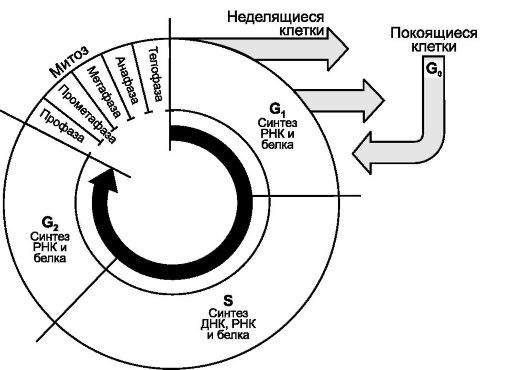
\includegraphics[width=0.5\linewidth]{pictures/cell_cykle}
\caption{Схема клеточного цикла}

\label{cell_cykle}
\end{figure}
%%%%%%%%%%%%%%%%%%%%%%%%%%%%%%%%%%%%%%%%%%%%%%%%%%%%%%%%%%%%%%%%%%%%%%%%%%%%%%%%%%%%%%%%%% 

\paragraph*{}\note{Клетки образовательных тканей находятся на эмбриональной стадии в течении всей своей жизни}

\subsubsection*{Фаза растяжения}

\paragraph*{}Прекратившие деление клетки переходят к росту путем \hypertarget{strainGrowth}{растяжения}. Процесс роста клетки растяжением можно описать следующей цепочкой событий:

\begin{enumerate}
	\item Под действием гормона \hyperlink{auxin}{ауксина} активируется транспорт протонов в \hyperlink{cell_wall}{клеточную стенку}
	\item \hyperlink{cell_wall}{Клеточная стенка} разрыхляется, становится более упругой, вследствие чего в \hyperlink{cell_vakuol}{центральную вакуоль} клетки начинает поступать вода.
	\item Растущая клетка начинает увеличиваться в размерах за счет образования большой \hyperlink{cell_vakuol}{центральной вакуоли} и формирования органелл и цитоплазмы. 
	\item В везикулах аппарата Гольджи из галактуроновой кислоты начинает синтезироваться пектин, а на наружной стороне плазмалеммы -- \hyperlink{cellulosa}{целлюлозные волокна}
	\item В \hyperlink{cell_wall}{клеточную стенку} начинают включатся новые волокна целлюлозы и пектиновые вещества. 
	\item В конце фазы растяжения усиливается лигнификация клеточных стенок, что снижает ее упругость и проницаемость, накапливаются ингибиторы роста, повышается активность оксидазы \gls{inodolAcid}, снижающей содержание \hyperlink{auxsin}{ауксина} в клетке.
\end{enumerate}

\subsubsection*{Фаза дифференцировки}

\paragraph*{}На данной стадии клетка приобретает морфологические и физиологические особенности, необходимые ей для дальнейшего функционирования в составе определенной ткани (\ris \ref{plants_cells}) В основе процессов дифференцировки лежит изменение активности или \gls{genExpression} различных генов. 

%%%%%%%%%%%%%%%%%%%%%%%%%%%%%%%%%%%%%%%%%%%%%%%%%%%%%%%%%%%%%%%%%%%%%%%%%%%%%%%%%%%%%%%%%%%%%%%%%%%%%%%%%%% 
\begin{figure}[h!]
  \centering
       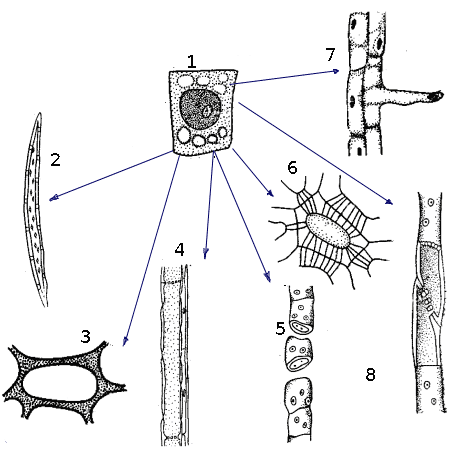
\includegraphics[width=0.5\linewidth]{pictures/plants_cells}
\caption{Различные типы растительных клеток}
\label{plants_cells}
\end{figure}
%%%%%%%%%%%%%%%%%%%%%%%%%%%%%%%%%%%%%%%%%%%%%%%%%%%%%%%%%%%%%%%%%%%%%%%%%%%%%%%%%%%%%%%%%% 

\paragraph*{}\remember{Сигналами для экспрессии только определенных генов служат сочетания фитогормонов, метаболитов и физико-химических факторов (например, давление соседних клеток)}

\paragraph*{}Таким образом, каждая клетка растения содержит в своем геноме полную информацию о развитии всего организма и, потенциально, может дать начало формированию целого растения. Данное свойство носит название \gls{totipatentia}. 

\paragraph*{}Однако, находясь в составе организма, эта клетка будет реализовать только часть своей генетической информации. 

\subsubsection*{Фаза зрелости} 

\paragraph*{}Зрелая клетка начинает выполнять функции, свойственные клеткам той \hyperlink{plants_tisues}{ткани}, в состав которой она входит.

\paragraph*{}\note{Некоторые ткани состоят из мертвых клеток. Такими тканями являются, например ксилема и склеренхима}

\subsubsection*{Старение и смерть}

\paragraph*{}Старение и смерть клетки происходит в результате:

\begin{enumerate}
\item Накопления повреждений в генетическом аппарате, клеточных мембранах и включениях;
\item Генетической програмированной клеточной; смерти\footnote{генетически запрграммированная смерть клеток животных называется апоптоз}
\end{enumerate}

\paragraph*{}При старении клеток происходит усиление процессов гидролиза входящих в состав клетки веществ и одновременное ослабление процессов синтеза новых веществ. В органеллах и цитоплазме образуются автофагические вакуоли, разрушаются \hyperlink{sect_hlorophilus}{хлорофилл} и \hyperlink{cell_plastids}{хлоропласты}, эндоплазматический ретикулум, аппарат Гольджи, ядрышко, набухают \hyperlink{mitohondria}{митохондрии}, в них снижается число крист, вакуолизируется ядро. 

\remember{Гибель клетки становится необратимой после разрушения \hyperlink{plasmolema}{клеточных мембран}, в том числе и \hyperlink{cell_vakuol}{тонопласта}, выхода содержимого вакуоли и лизосом в цитоплазму}

\subsection*{Этапы онтогенеза высших растений} 

\paragraph*{}Каждый растительный организм в своем \hypertarget{plant_ontogenesis}{развитии} проходит ряд этапов, характеризующихся морфологическими и физиологическими особенностями.

%%%%%%%%%%%%%%%%%%%%%%%%%%%%%%%%%%%%%%%%%%%%%%%%%%%%%%%%%%%%%%%%%%%%%%%%%%%%%%%%%%%%%%%%%%%%%%%%%%%%%%%%%%% 
\begin{figure}[h!]
  \centering
       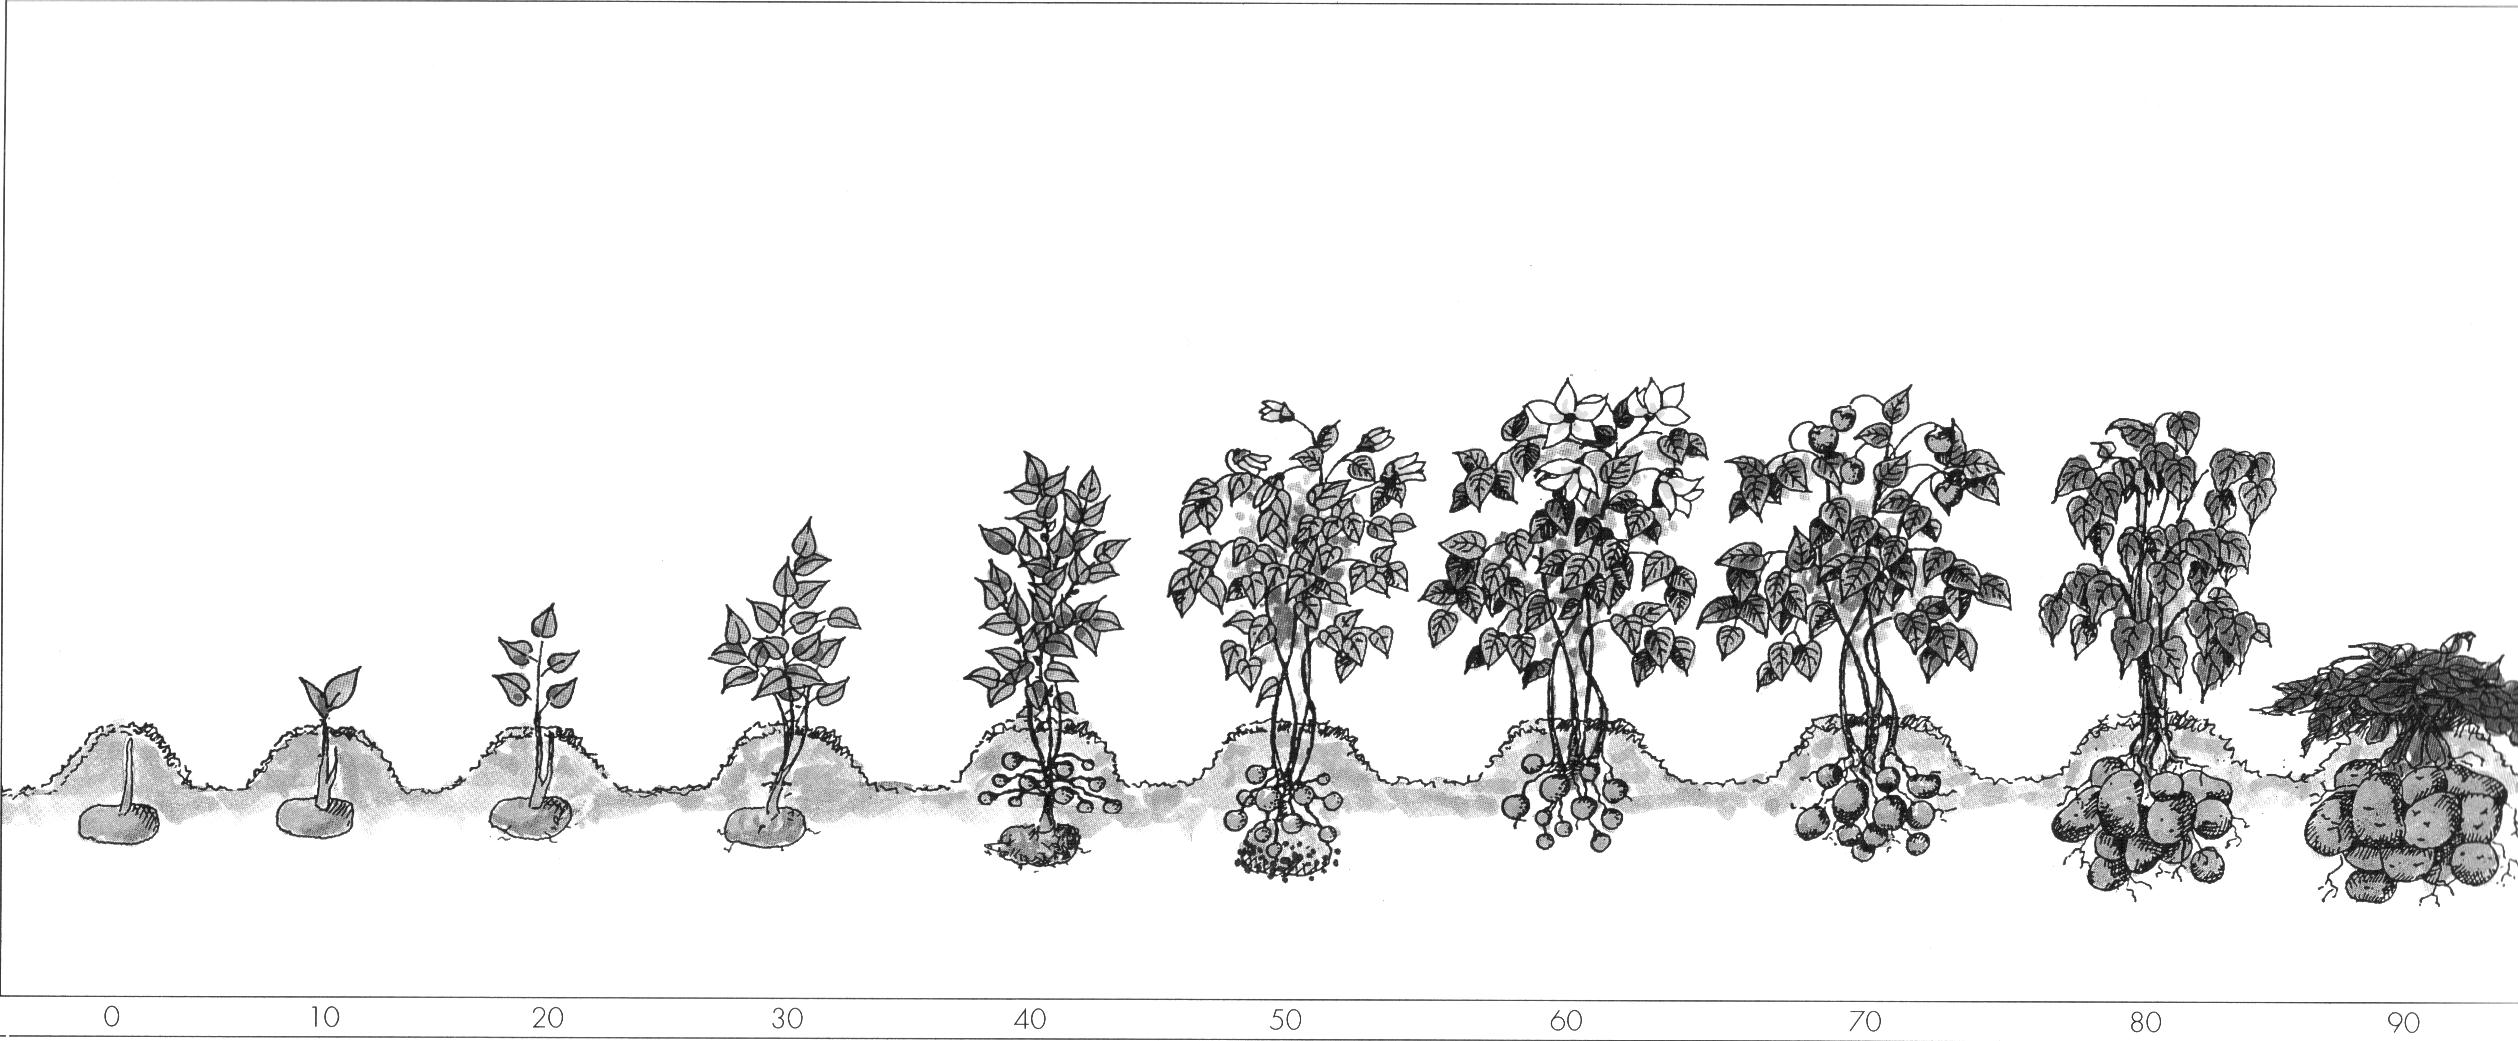
\includegraphics[width=0.7\linewidth]{pictures/ontogenesis_stages}
\caption{Этапы онтогенеза растения}
\label{ontogenesis_stages}
\end{figure}
%%%%%%%%%%%%%%%%%%%%%%%%%%%%%%%%%%%%%%%%%%%%%%%%%%%%%%%%%%%%%%%%%%%%%%%%%%%%%%%%%%%%%%%%%% 

\subsubsection*{Ювенильный этап} 

\paragraph*{}Ювенильный этап (\ris \ref{ontogenesis_stages}) начинает с прорастания семян или органов вегетативного размножения и характеризуется накоплением вегетативной массы. Растения на этом этапе не способны к половому размножению.

\subsubsection*{Этап зрелости и размножения}

\paragraph*{}Зрелое (взрослое) растение способно к половому размножению. Происходит формирование генеративных органов и образование плодов. 
\paragraph*{}У растений выделяют следующие типы размножения:

\begin{enumerate}
	\item \gls{sexualMaturing}, когда новый организм появляется в результате слияния половых клеток -- гамет;
	\item \gls{asexualMaturing}, когда новый организм развивается из спор;
	\item \gls{vegetationMaturing} -- воспроизведение растений из вегетативных частей растения (клубней, луковиц, отводок)
\end{enumerate};

%\paragraph*{}\note{Бесполое размножение характерно для споровых растений}

\paragraph*{}\gls{life_cycle} всех растений характеризуется чередованием двух поколений -- гаплоидного \gls{gametophit}а и диплоидного \gls{sporophit}а. При этом, эволюция растений была направлена в сторону постепенной редукции гаметофита. Так, у споровых растений гаметофит и спорофит являются самостоятельными организмами. У семянных же растений гаметофит утратил самостоятельность, женский гаметофит существует в виде семязачатка внутри завязи цветка, а мужской гаметофит -- это пыльцевое зерно (\ris \ref{life_cycle} б).

%%%%%%%%%%%%%%%%%%%%%%%%%%%%%%%%%%%%%%%%%%%%%%%%%%%%%%%%%%%%%%%%%%%%%%%%%%%%%%%%%%%%%%%%%%%%%%%%%%%%%%%

\begin{figure}[h]
\begin{minipage}[h]{0.49\linewidth}
\center{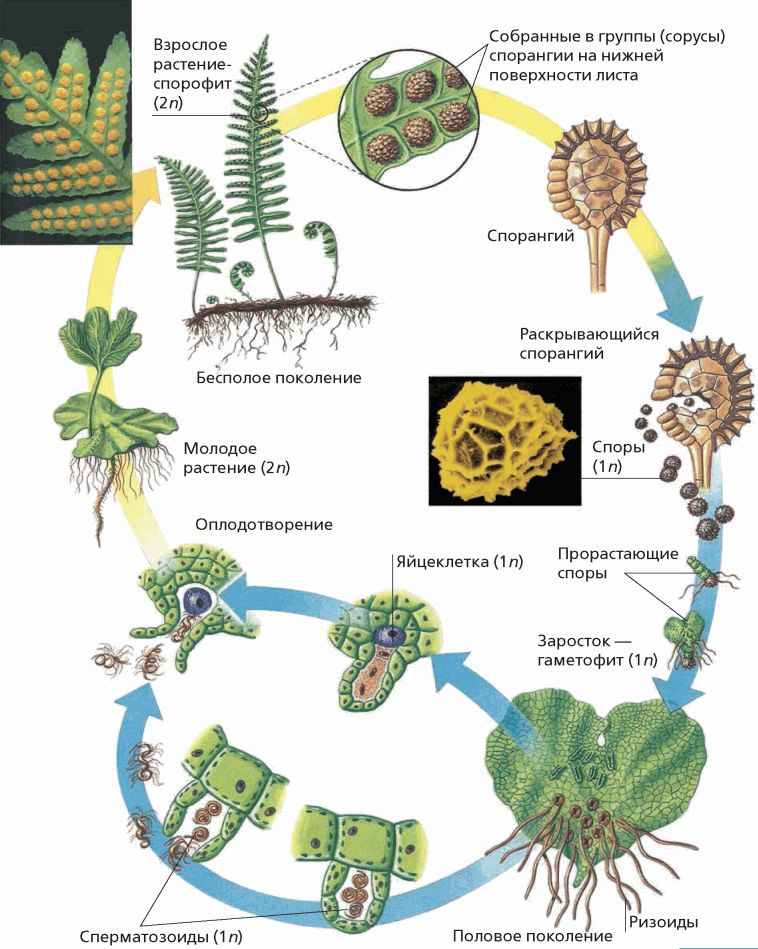
\includegraphics[width=0.9\linewidth]{pictures/i_103} \\ а) Папоротники}
\end{minipage}
\hfill
\begin{minipage}[h]{0.49\linewidth}
\center{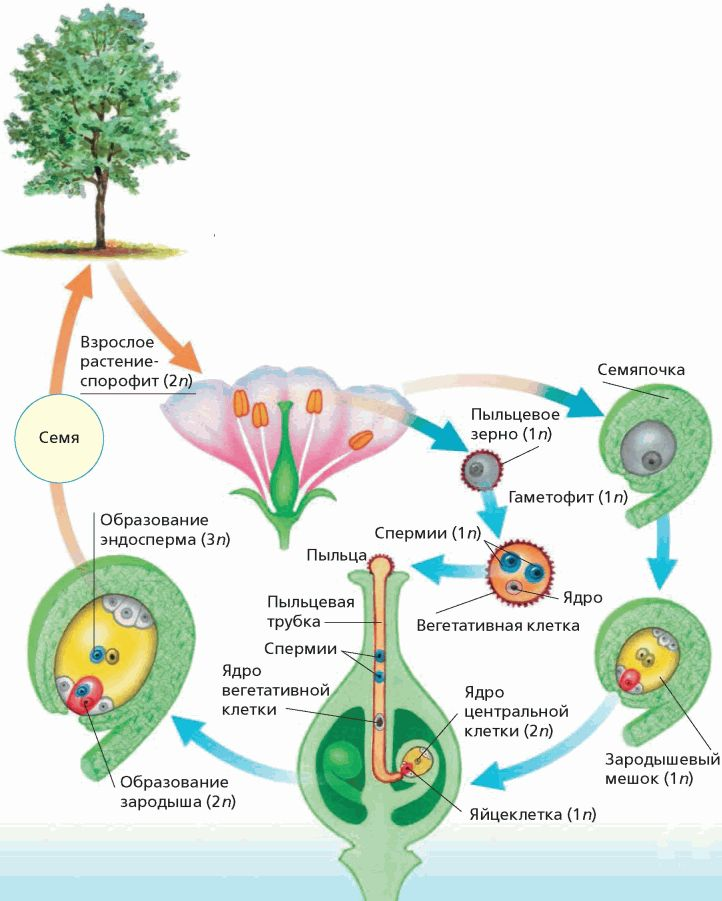
\includegraphics[width=0.9\linewidth]{pictures/i_125} \\ б) Цветковые растения}
\end{minipage}
\caption{Схема жизненного цикла споровых и цветковых растений}
\label{life_cycle}
\paragraph*{}Схема взята из \cite{sonin_bio}
\end{figure}

%%%%%%%%%%%%%%%%%%%%%%%%%%%%%%%%%%%%%%%%%%%%%%%%%%%%%%%%%%%%%%%%%%%%%%%%%%%%%%

\paragraph*{}В зависимости от количества циклов полового размножения в жизненном цикле, все растения делятся на две большие группы: 

\begin{enumerate}
	\item \gls{monokarpics} (плодоносящие один раз). К монокарпическим относятся все однолетние растения, некоторые двулетние и многолетние.
	\item \gls{polykarpics} (плодоносящие многократно). Большинство многолетних растений
\end{enumerate}

\paragraph*{}Среди монокарпических растений выделяют такие жизненные формы, как

\begin{enumerate}
	\item \gls{ephemers} -- растения, \gls{life_cycle} которых занимает всего несколько недель
	\item Однолетники (яровые и озимые злаки, картофель, бобовые)
	\item Двулетники (корнеплоды, капуста, лук)
	\item Многолетники (агавы, некоторые пальмы)
\end{enumerate} 

\paragraph*{}В свою очередь, серди поликарпических растений выделяют виды, цветущие на \cite{rubin_71}:

\begin{enumerate}
	\item 1-ый год жизни (ряд многолетних злаков);
	\item 2-ой год жизни (люцерна, многолетний люпин);
	\item 3-ий год жизни (ягодные кустарники);
	\item 8-12 год жизни (яблоня, груша);
	\item 25-30 год жизни (липа, клен);
	\item 40-60 год жизни (дуб);
\end{enumerate}

\paragraph*{}Инициация перехода к цветению осуществляется под действием внешних факторов, таких как температура (\gls{jarovisation}), чередование дня и ночи (\gls{photoperiodism}) или эндогенных факторов, обусловленных возрастом растения. Растения, нуждающиеся в яровизации, называют озимыми, а развивающиеся без нее -- яровыми. 

%Яровизация – это неизвестный пока процесс, протекающий в растениях под действием низких положительных температур и способствующий последующему ускорению развития растений. 
\note{Различия между озимыми и яровыми формами зерновых культур обусловлены генетически. Так, озимая и яровая рожь различаются всего по одному гену}

\paragraph*{}В зависимости от реакции на длину дня, растения делятся на

\begin{enumerate}
	\item Короткодневные, переходящие к цветению только тогда, когда день короче ночи (рис, соя);
	\item Длиннодневные (хлебные злаки, крестоцветные, укроп); 
	\item Растения, нуждающиеся в чередовании разных фотопериодов, а также 
	\item Нейтральные по отношению к длине дня (гречиха, горох);
\end{enumerate}

\note{Длиннодневные растения распространены, в основном, в умеренных и приполярных широтах, короткодневные -- в субтропиках}

\paragraph*{}У большинства растений наибольшей чувствительностью к фотопериоду обладают листья, только что закончившие рост. Основную роль в восприятии фотопериода играет белок \hyperlink{phitochrom}{фитохром}, который под действием света может менять свою конформацию.

%Показано участие в переходе к цветению стимулятора роста гиббереллина. В условиях неблагоприятного фотопериода в листья обнаруживаются ингибиторы цветения. 
\paragraph*{}Цветы -- это органы полового размножения (\gls{generativeOrgans}). Цветки как органы полового размножения могут быть обоеполыми или раздельнополыми. Они формируются на одних и тех же (однодомность) или на разных (двудомность) растениях. 

\paragraph*{}Факторы внешней среды, приводящие к увеличению содержания в растении цитокининов и \hyperlink{auxsin}{ауксинов}, увеличивают долю женских цветков, а повышающие концентрацию гиббереллинов -- мужских.

\paragraph*{Двойное оплодотворение}

\paragraph*{}Одной из особенностей цветковых растений является двойное оплодотворение. При этом, в процессе оплодотворения выделяют три фазы:

\begin{enumerate}
	\item Опыление, когда пыльцевое зерно попадает на рыльце пестика;
	\item Прорастание пыльцы и рост пыльцевой трубки в тканях пестика;
	\item Собственно оплодотворение, то есть образование зиготы;
\end{enumerate}

\paragraph*{}При двойном оплодотворении зигота образуется при слиянии спермия пыльцевой трубки (мужской \gls{gametophit}) с яйцеклеткой зародышевого мешка (женский \gls{gametophit}). В это же время, второй спермий соединяется с вторичным диплоидным ядром центральной клетки зародышевого мешка. 
%Зародыши проходят ряд последовательных фаз развития. На последнем этапе созревания семена теряют значительное количество воды и переходят в состояние покоя, когда в тканях уменьшается содержание стимуляторов роста и увеличивается количество ингибитора роста абсцизовой кислоты.

\paragraph*{}Плод развивается из завязи цветка и, как правило, содержит семена. Плоды могут формироваться без оплодотворения и образования семян. Это явление называется \gls{partenokarpia}. Образование партенокарпических (бессемянных) плодов может происходить при обработке растений \hyperlink{auxsin}{ауксинами} и гиббереллинами. Однако обычно цветки без опыления и оплодотворения опадают.

\subsubsection*{Этап старости и отмирания}

\paragraph*{}Этап старости и отмирания (\ris \ref{ontogenesis_stages}) включает в себя период от полного прекращения плодоношения до смерти организма. Для него характерно прогрессирующее ослабление жизнедеятельности. 

\paragraph*{}У многих растений периодически отмирают отдельные элементы побега:
\begin{enumerate}
	\item Однолетние растения погибают целиком;
	\item У многолетних трав ежегодно полностью отмирает надземная часть, а корневая система остается жизнеспособной;
	\item У многих растений стареют и опадают ранее образовавшиеся листья;
	\item У листопадных деревьев осенью одновременно стареют и опадают все листья одновременно. 
\end{enumerate}

\paragraph*{}Перед опадением листа или плода в основании черешка листа или плодоножки образуется отделительный слой -- зона, где у клеток размягчаются и частично растворяются клеточные стенки и срединные пластинки. Этот процесс начинается под воздействием этилена, который вырабатывается стареющими листьями и созревающими плодами.

\subsection*{Дифференцировка и рост растений}

\paragraph*{}У животных в течение жизни происходит лишь увеличение размеров заложенного перед рождением органа, а у растений -- заложение и увеличение размеров органа идет параллельно в течение всего онтогенеза

\remember{Характерной  чертой растений является то, что новые ткани и органы растений формируются за счет деятельности специальной образовательной ткани, которая носит название \gls{meristema}}

\paragraph*{}Существование меристем поддерживается инициальными клетками \gls{initialCells}, длительное время способными к делению путем митоза. 

\note{У мхов, хвощей и папоротников в апикальной меристеме имеется только одна инициалия в виде трехгранной пирамиды с выпуклым основанием, у других высших растений инициалий несколько и они трудноотличимы от остальных клеток \gls{apex}а \cite{korowkin_gloss}}.

\paragraph*{}Более длительная способность к делению является следствием меньшей частоты делений и большей длительности интерфазы.

\paragraph*{}Различают следующие типы меристем:

\begin{enumerate}
	\item Апикальные (верхушечные) \gls{meristema} расположены на концах побегов и корней --\gls{apex}ах (\ris \ref{apex}). Апикальные меристемы побега и корня представляют собой не только образовательные ткани, но и главные координирующие центры влияющие на морфогенетические процессы в целом растении;
	\note{Так как кончики растущего корня или стебля первыми ощущают на себе действие факторов окружающей среды, в них расположены многие рецепторные системы растения}
	\item Латеральные (боковые) \gls{meristema} образуют слои клеток вдоль побега и корня В результате деления клеток камбия образуются ксилема и флоэма;
	\item Интерколлярные или вставочные \gls{meristema} -- расположены в основании междоузлий и листьев;
\end{enumerate}

%%%%%%%%%%%%%%%%%%%%%%%%%%%%%%%%%%%%%%%%%%%%%%%%%%%%%%%%%%%%%%%%%%%%%%%%%%%%%%%%%%%%%%%%%%%%%%%%%%%%%%%%%%% 
\begin{figure}[h!]
  \centering
       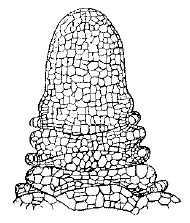
\includegraphics[width=0.3\linewidth]{pictures/apex}
\caption{Апекс побега эллодеи}
\paragraph*{}Рисунок приведен согласно \cite{korovkin_2007}
\label{apex}
\end{figure}
%%%%%%%%%%%%%%%%%%%%%%%%%%%%%%%%%%%%%%%%%%%%%%%%%%%%%%%%%%%%%%%%%%%%%%%%%%%%%%%%%%%%%%%%%% 


\paragraph*{}\gls{morphogenesis}, то есть формообразование у растений включает в себя процессы заложения, роста и развития

\begin{enumerate}
	\item Клеток (цитогенез);
	\item Тканей (гистогенез);
	\item Оганов (органогенез);
\end{enumerate}
\remember{Процессы морфогенеза генетически запрограммированы и скоординированы между собой} 

%Межклеточные системы регуляции включают гормональные, электрические и трофические факторы, которые влияют на генетическую, мембранную и метаболическую регуляторные системы в каждой клетке. 

\paragraph*{}Включение и выключение генетических программ в клетке зависит от поступления в клетку сигналов, особенно \hyperlink{gormons}{фитогормонов}, из других клеток. 

%Ауксин необходим для включения генетической программы корнеобразования, а цитокинин в присутствии ауксина вызывает экспрессию генов, ответственных за программу побегообразования.
\paragraph*{}В процессе морфогенез растительного организма наблюдается поляризация развития отдельных структур. \gls{polarisation} биологических структур -- это ориентация процессов и структур в пространстве, то есть физиолого-биохимические и анатомо-морфологические свойства изменяются в определенном направлении. 

\paragraph*{}\gls{polarisation} вызывается:

\begin{enumerate}
	\item Градиентами осмотического давления;
	\item pH;
	\item Концентрации кислорода и углекислого газа;
	\item Гормональными, электрическими и трофическими контактами с соседними клетками;
	\item Механическим давлением;
\end{enumerate}

%\paragraph*{}В результате в клетках реализуются именно те потенции, которые соответствуют окружающим условиям. 

\note{У растительных клеток найдены рецепторы фитогормонов, позволяющие клеткам <<ощущать>> наличие гормонов в окружающей среде. При культивировании клеток в искусственной среде проявляется так называемый <<эффект массы>>. Он выражается в том, что единичная изолированная клетка редко переходит к делению. Чем гуще суспензия клеток, тем большее их число начинает делиться. Для дифференциации большое значение имеет наличие в клеточной стенке белков лектинов, участвующих в узнавании и взаимодействии клеток}

\paragraph*{}В процессе роста наблюдается также зависимость роста и развития одних органов от других -- \gls{growthCorrelations}. 

\note{Например, очевидно, что развитие побега зависит от корня, поставляющего минеральные вещества и воду. В свою очередь, побег поставляет в корень органические соединения. По этой причине, площадь коневой системы дерева сопоставима с площадью его кроны} 

\paragraph*{}Основную роль в процессе роста играют гормональные взаимодействия между частями растения. 

\note{Примером гормональной регуляции служит явление апикального доминирования, которое заключается в торможении верхушкой побега или корня развития соответственно пазушных почек или боковых корней}

\paragraph*{}\gls{apexDominance} доминирование обусловлено тем, что:

\begin{enumerate}
	\item Точка роста побега, содержащая большое количество \hyperlink{auxsin}{ауксина}, является мощным центром, притягивающим питательные вещества и гормон \hyperlink{citokin}{цитокин} синтезированный в корне;
	\item \hyperlink{auxsin}{Ауксин} задерживает образование проводящих пучков, соединяющих боковые почки с центральной проводящей системой;
\end{enumerate}

\paragraph*{}\gls{apexDominance} исчезает при удалении апекса центрального побега. После этого начинается интенсивный рост боковых побегов.

%Удаление верхушки побега стимулирует этот процесс, а приток цитокинина к пазушным почкам усиливает в них клеточные деления. Формирующиеся в боковых почках листовые зачатки начинают синтезировать ауксин, необходимый для дальнейшего развития боковых побегов.

\note{Ростовые корреляции используются в растениеводстве для получения большего количества продукции. Например, пасынкование -- удаление боковых побегов у томатов способствует образованию более крупных плодов, пикировка -- обрывание кончиков корней при пересадке рассады овощей увеличивает число боковых корней}

\paragraph*{}Процессам роста, как и другим физиологическим явлениям, свойственна периодичность, которая вызывается как особенностями самих процессов, так и факторами внешней среды. 

\paragraph*{}Наиболее распространены в организме растения процессы с периодичностью около суток. К таким процессам относятся 

\begin{enumerate}
\item Изменения митотической активности в меристемах
\item \hyperlink{photosyntesis}{Фотосинтез}
\item \hyperlink{sect_breazing}{Дыхание}
\item Открытие и закрытие цветков
\end{enumerate}

\paragraph*{}Суточные ритмы связаны с суточными колебаниями освещенности и температуры. 

\paragraph*{}Кроме суточной для растений характерна сезонная периодичность, заключающаяся в наступлении периодов покоя. Различают следующие типы покоя:

\begin{enumerate}
\item \gls{necessityRepose}, обусловленный факторами внешней среды, препятствующими прорастанию;
\item Физиологический покой (глубокий покой), который регулируется балансом стимуляторов и ингибиторов роста
\end{enumerate}

%При вступлении в период покоя происходят процессы, повышающие устойчивость клеток к неблагоприятным факторам среды: возрастает вязкость цитоплазмы, она отходит от клеточных стенок, что нарушает связь между клетками, снижается интенсивность процессов обмена. Сухие семена не прорастают до тех пор, пока не будет достаточного количества воды. Весной почки не распускаются, пока не поднимется до определенного уровня температура. 

\paragraph*{}Из состояния вынужденного покоя растение выходит как только условия окружающей среды становятся благоприятными.

\paragraph*{}Растения, находящиеся в физиологическом покое, не переходят к росту даже при благоприятных условиях среды. Для выхода семян из глубокого покоя их подвергают стратификации. \gls{stratification} заключается в выдерживании влажных семян при пониженной температуре.

%\subsection*{Регенерация у растений} 

%Регенерация – это восстановление организмом поврежденной или утраченной части тела, что является одним из способов вегетативного размножения и защиты растений от повреждений. Различают следующие виды регенерации.
%I. Физиологическая регенерация.
%Части восстанавливаются при их естественном изнашивании, например, постоянное восполнение слущивающихся клеток корневого чехлика.
%II. Травматическая регенерация.
%1. Регенерация, обусловленная дедифференцировкой клеток:
%а) заживление ран.
%Эпидермис и первичная кора дедифференцируются, их клетки начинают делиться и образуют вторичную меристему, которая превращается в пробку.
%б) органогенез, связанный с образованием каллуса.
%Клетки дедифференцируются и переходят к неорганизованному делению, образуя каллусную ткань из рыхло соединенных друг с другом паренхимных клеток. Иногда отдельные клетки дают начало адвентивным, то есть возникшим не из эмбриональных тканей, органам: корням, побегам, листьям.
%в) соматический эмбриогенез.
%На раневой поверхности образуется каллус. Из отдельных клеток каллуса, начинающих делиться, формируются соматические зародыши (эмбриоиды), из которых при определенных условиях развивается целый организм.
%г) восстановление частей без образования каллуса.
%Паренхимные клетки коры под влиянием ауксина, индуцирующего генетическую программу ксилемообразования, превращаются в клетки ксилемы при образовании обходного участка проводящего пучка вокруг места его прерывания.
%2). Регенерация на уровне меристем:
%а) восстановление апикальных меристем.
%При продольном рассечении конуса нарастания из каждой половины могут регенерировать отдельные апексы.
%б) органогенез из предсуществующих зачатков.
%Восстановление надземных органов у высших растений происходит за счет отрастания пазушных почек при устранении доминирующего влияния апекса побега.

\subsection*{Кинетика ростовых процессов} 

\paragraph*{}Кривую, описывающую скорость роста, можно разделить на 4 участка (\ris \ref{growth_line}): 

\begin{enumerate}
	\item Лаг-период -- рост почти не заметен и идут процессы, подготавливающие организм к видимому росту;
	\item Лог-фаза -- скорость роста изменяется логарифмически;
	\item Фаза замедления роста;
	\item Стационарная фаза;
\end{enumerate}

%%%%%%%%%%%%%%%%%%%%%%%%%%%%%%%%%%%%%%%%%%%%%%%%%%%%%%%%%%%%%%%%%%%%%%%%%%%%%%%%%%%%%%%%%%%%%%%%%%%%%%%%%%% 
\begin{figure}[h!]
  \centering
       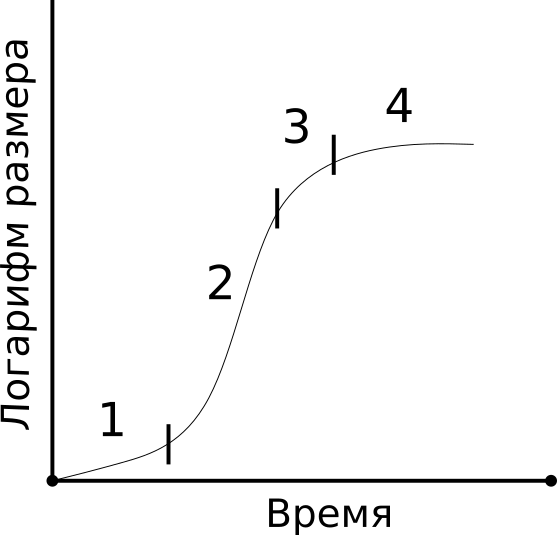
\includegraphics[width=0.5\linewidth]{pictures/growth_line}
\caption{Кривая роста}
\label{growth_line}
\end{figure}
%%%%%%%%%%%%%%%%%%%%%%%%%%%%%%%%%%%%%%%%%%%%%%%%%%%%%%%%%%%%%%%%%%%%%%%%%%%%%%%%%%%%%%%%%% 

%1 – лаг-период, 2 – логарифмическая фаза, 3 – фаза замедленного роста, 4 – фаза стационарного состояния (по С. И. Лебедеву).

\paragraph*{}Для измерения скорости роста используются следующие показатели.

\paragraph*{}\gls{growthRate} r -- прирост массы растения или отдельного его органа в единицу времени, который рассчитывается по формуле Блекмана \ref{blekman} \cite{malinowsky_2004}

\begin{equation}
	r=\frac{\lg{\frac{W_{1}}{W_{0}}}} x 2,3026
		{t}
		\label{blekman}
\end{equation}
   
\paragraph*{}где $W_{0}$ – начальный, а $W_{1}$ – конечный вес сухого вещества, t – промежуток времени между определениями.

\paragraph*{}\gls{relativeGrowthRate} R -- прирост, вычисленный в процентах от исходного веса растения или органа \ref{relative_growth}:            

\begin{equation}
	R=\frac{W_{1}-W_{0}}{W_{0}} x 100
	\label{relative_growth}
\end{equation}

\paragraph*{}\gls{absoluteGrowthRate} К -- величина прироста за промежуток времени, отнесенная к единице времени \ref{absolute_growth}:

\begin{equation}
	K=\frac{W_{2}-W_{1}}{t_{2}-t_{1}}
	\label{absolute_growth}
\end{equation}


\subsection*{Влияние факторов внешней среды на рост растений}

На рост растений оказывают влияние такие факторы, как

\begin{enumerate}
	\item Продукты жизнедеятельности одних растений могут подавлять рост других -- аллелопатия;
	\item Продукты жизнедеятельности микроорганизмов (антибиотики, регуляторы роста) 
	\item Факторы внешней среды, такие как температура воздуха, уровень освещенности и т.д.
\end{enumerate} 

\subsubsection*{Свет}

\paragraph*{}Растения воспринимают свет не только как источник энергии, но и в качестве сигнала, характеризующего условия среды. Растение воспринимают изменение длинны светового дня с помощью специальных молеку-рецепторов -- \hypertarget{phitochrom}{фитохрома}, опосредующего действие света на морфогенез. \gls{phitochrom} состоит из двух белковых субъединиц и хромофора – незамкнутого тетрапиррола, относящегося к группе фикобилинов. \gls{phitochrom} синтезируется в форме, поглощающей красный свет (Ф660). Под действием красного света эта форма фитохрома переходит в активную форму, поглощающей дальний красный свет (Ф730). Под действием дальнего красного света и в темноте Ф730 превращается обратно в Ф660. 
\paragraph*{}Фитохром оказывает на клетку следующие физиологическое воздействие: 

\begin{enumerate}
	\item Изменяет проницаемость \hyperlink{plasmolema}{клеточных мембран};
	\item Регулирует движение \hyperlink{cell_plastids}{хлоропластов};
	\item Влияет на синтез ферментов и стимуляторов роста \hyperlink{gybberelin}{гиббереллинов} и \hyperlink{citokin}{цитокининов};
\end{enumerate}

\subsubsection*{Температура}

\paragraph*{}Различают три основные температурные точки: 

\begin{enumerate}
	\item Минимальная температура, при которой начинается рост растения;
	\item Оптимальная температура, наиболее благоприятная для роста растения;
	\item Максимальная, при которой рост растения прекращается;
\end{enumerate}

\paragraph*{}В зависимости от приспособленности к температурному режиму различают:

\begin{enumerate}
	\item Теплолюбивые растения (минимальная температура выше 10~ \celsius, оптимальная 30-40~ \celsius)
	\item Холодостойкие растения (минимальная температура 0-5~ \celsius, оптимальная 25-30~ \celsius)
\end{enumerate}


%\subsubsection*{Газовый состав атмосферы}
%Газовый состав. Необходим кислород, так как дыхание поставляет энергию для ростовых процессов, и углекислый газ, который в ходе фотосинтеза восстанавливается до органических веществ. Избыток углекислого газа на короткое время повышает растяжимость клеточных стенок и стимулирует рост клеток (эффект «кислого роста»).

\subsubsection*{Водный режим}
\paragraph*{}Недостаточное снабжение растений водой задерживает рост побегов и кратковременно стимулирует с последующим торможением рост корней. 

\subsubsection*{Минеральное питание}
\paragraph*{}Для нормального роста необходимо достаточное снабжение всеми питательными элементами. 
%Избыток азота стимулирует рост вегетативной массы, но замедляет процессы дифференцировки и формирование цветков.

\subsection*{Фитогормоны} 

\paragraph*{}\hypertarget{gormons}{\gls{phitogormons}} образуются в процессе обмена веществ растений и оказывают в очень малых количествах регуляторное и координирующее влияние на физиологические процессы в разных органах. Различают стимуляторы и ингибиторы роста. 

\remember{Следует помнить, что стимуляторы роста, применяемые в сверхоптимальных дозах, способны подавлять ростовые процессы}

\subsubsection*{Ауксины}

\paragraph*{}Главным представителем \hypertarget{auxsin}{\gls{auxin}ов} в растениях является \gls{inodolAcid} (\ris \ref{growth_stimulators}) Она синтезируется из триптофана в верхушке побега. Разрушается \gls{inodolAcid} ферментом ИУК-оксидазой. 

\paragraph*{}Ауксин оказывает стимулирующие влияние на следующие процессы, происходящие в растении:

\begin{enumerate}
	\item Стимулирует деление и растяжение клеток;
	\item \gls{inodolAcid} активирует протонную помпу в плазмалемме, что приводит к закислению и разрыхлению \hyperlink{cell_wall}{клеточной стенки} во время роста клетки за счет \hyperlink{strainGrowth}{растяжения};
	\item Необходим для образования проводящих пучков и корней;
	\item Комплекс \gls{inodolAcid} с рецептором транспортируется в ядро и активирует синтез \gls{rna}, что в свою очередь, приводит к усилению \hyperlink{proteinSintez}{синтеза} \hyperlink{proteins}{белков};
\end{enumerate}

%%%%%%%%%%%%%%%%%%%%%%%%%%%%%%%%%%%%%%%%%%%%%%%%%%%%%%%%%%%%%%%%%%%%%%%%%%%%%%%%%%%%%%%%%%%%%%%%%%%%%%%

\begin{figure}[h]
\begin{minipage}[h]{0.49\linewidth}
\center{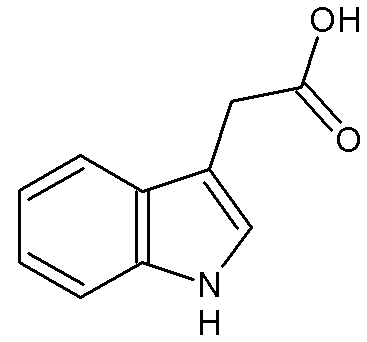
\includegraphics[width=0.7\linewidth]{pictures/auxin} \\ а) Ауксин}
\end{minipage}
\hfill
\begin{minipage}[h]{0.49\linewidth}
\center{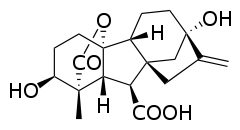
\includegraphics[width=0.9\linewidth]{pictures/gibberelin} \\ б) Гибберелин}
\end{minipage}
%\caption{Зависимость сигнала от шума для данных.}
\label{growth_stimulators}
\end{figure}

%%%%%%%%%%%%%%%%%%%%%%%%%%%%%%%%%%%%%%%%%%%%%%%%%%%%%%%%%%%%%%%%%%%%%%%%%%%%%%

\subsubsection*{Цитокинины}
\paragraph*{}\hypertarget{citokin}{Цитокинины} образуются путем конденсации аденозин-5-монофосфата и изопентенилпирофосфата в апикальной меристеме корня. Много цитокининов в развивающихся семенах и плодах. 
\paragraph*{}Цитокины стимулируют следующие процессы:

\begin{enumerate}
	\item В присутствии вызывает \hyperlink{auxsin}{ауксина} деление клеток;
	\item Активируют дифференциацию \hyperlink{cell_plastids}{пластид};
	\item Повышают активность АТФ-синтетазы;
	\item Способствуют выходу почек, семян и клубней из состояния покоя;
	\item Предотвращают распад \hyperlink{sect_hlorophilus}{хлорофилла} и деградацию клеточных органелл;
	\item Комплекс цитокининов с белковым рецептором повышает активность \gls{rna}-полимеразы. При повышается \gls{genExpression} этом увеличивается число полисом и активируется синтез белка;
\end{enumerate}

\subsubsection*{Гиббереллины}

\note{В настоящее время известно более 70 \hypertarget{gybberelin}{гиббереллинов} кислой и нейтральной природы} 

\paragraph*{}Наиболее известным и распространенным гиббереллином является гибберелловая кислота (\ris \ref{growth_stimulators}). Исходным веществом для синтеза гибберелинов является \gls{acetylCoensimA}. \gls{gibberelins} синтезируются  в листьях и корнях. 

\paragraph*{}\gls{gibberelins} способствуют:

\begin{enumerate}
	\item Удлинению стебля;
	\item Выходу семян из состояния покоя;
	\item Формированию гранулярного эндоплазматического ретикулума;
	\item Образованию цветоноса и цветению;
	\item Активируют деление клеток в апикальных и интеркалярных меристемах;
	\item Повышают активность \hyperlink{enzimes}{ферментов} синтеза \hyperlink{plipids}{фосфолипидов};
	\item Комплекс гиббереллина с белковым цитоплазматическим рецептором стимулирует синтез нуклеиновых кислот и \hyperlink{proteins}{белка};
\end{enumerate}

\subsubsection*{Абсцизовая кислота}

\paragraph*{}Cинтезируется в листьях и корневом чехлике двумя путями: из мевалоновой кислоты или путем распада каротиноидов. \hypertarget{abscizeAcid}{\gls{abscizeAcid}} тормозит рост растений и является антагонистом стимуляторов роста. 

\paragraph*{}\note{Однако у огурца \gls{abscizeAcid} активирует удлинение гипокотиля, а у черенков фасоли образование корней} 

\paragraph*{}\gls{abscizeAcid} ускоряет распад нуклеиновых кислот, белков, \hyperlink{sect_hlorophilus}{хлорофилла}, ингибирует мембранную протонную помпу. 

\paragraph*{}\gls{abscizeAcid} накапливается в клетках

\begin{enumerate}
	\item При неблагоприятных условиях внешней среды;
	\item В стареющих листьях;
	\item В покоящихся семенах;
	\item В отделительном слое черешков листьев и плодоножек;
\end{enumerate}

\subsubsection*{Этилен}

\paragraph*{}Газ \hypertarget{eten}{этилен} синтезируется из метионина или путем восстановления ацетилена. Много этилена накапливается в стареющих листьях и созревающих плодах. 

\paragraph*{}Этилен вызывает следующие физиологические эффекты:

\begin{enumerate}

	\item Тормозит рост стеблей и листьев;
	\item Изменяет направление роста клеток с продольного на поперечное, что приводит к утолщению стебля;
	\item Ускоряет образование корней;
	\item Ускоряет созревание плодов, прорастание пыльцы, семян, клубней и луковиц.

\end{enumerate}

\subsubsection*{Брассиностероиды}

\paragraph*{}Брассиностероиды содержатся в разных органах растений, но особенно много их в пыльце. Они стимулируют рост в длину и толщину проростков, усиливая как деление, так и растяжение клеток.

\subsubsection*{Синтетические регуляторы роста}

\paragraph*{}Различают следующие типы синтетических регуляторов роста:

\begin{enumerate}

\item \gls{retardants} ингибируют рост стебля благодаря торможению растяжения клеток и подавлению синтеза гиббереллинов. Стебли становятся более короткими и утолщаются, в результате повышается устойчивость растения к полеганию.
\item \gls{morphactins} препятствуют прорастанию семян, образованию и росту побегов, ослабляют апикальное доминирование у побегов и усиливают его у корней.
\item Гербициды служат для уничтожения растительности. 
\note{Есть гербициды общего действия, когда погибают все растения, и селективные для избирательного уничтожения определенных классов растений. Они могут подавлять \hyperlink{photophosforolysis}{фотосинтетическое} или \hyperlink{photophosforolysis}{окислительное} фосфорилирование}
\item \gls{depholiants} ускоряют листопад у растений, что активирует созревание семян и плодов и облегчает механизированную уборку урожая.
\item Десиканты вызывают ускоренное высушивание листьев и стеблей, что позволяет вести сбор семенников бобовых культур и уборку картофеля комбайнами.
\item Сениканты – смесь физиологически активных веществ, вызывающих ускорение созревания и старения сельскохозяйственных растений

\end{enumerate}

\subsection*{Вопросы и задания для самоконтроля}

\begin{enumerate}
\item Приведите примеры, когда у растения происходит \hypertarget{rapid_growth}{быстрый рост пр}и медленном развитии?
\item Воспользуйтесь учебником общей биологии, например учебником Грина \cite{green_bio} и повторите тему <<\hypertarget{question_gen_code}{Генетический код}>>. Каким образом в молекуле \gls{dna} хранится наследственная информация?
\item На какой стадии своего развития клетка способна к делению?
\item Клетки какой ткани все время находятся на эмбриональной стадии развития?
\item Воспользуйтесь учебником общей биологии повторите тему <<Клеточный цикл>>. Сравните деление клетки \hypertarget{question_mitosis}{митозом} и мейозом. В чем сходство и в чем различие этих способов деления? Какие клетки делятся путем мейоза?
\item Какие типы \hypertarget{plants_tisues}{тканей} растения вы знаете, по каким характерным чертам различаются клетки той или иной ткани?
\item Какие факторы окружающей среды способны привести к нарушениям в генотипе?
\item Какие растения относятся к высшим споровым?
\item В жизненном цикле каких растений преобладает \gls{gametophit}, а \gls{sporophit} представлен коробочкой на ножке?
\item Если клетки-инициалии долгое время способны поддерживать деление митозом, то на какой стадии развития они находятся?
\item Какую роль в \hypertarget{proteinSintez}{синтезе} белка играет \gls{rna}
\item Назовите основные этапы онтогенеза злаковых.
\end{enumerate}